\documentclass{article}
\usepackage[utf8]{inputenc}
\usepackage[T2A]{fontenc}
\usepackage[english,russian]{babel}
\usepackage[left=1.5cm,right=1.5cm,top=2cm,bottom=2cm]{geometry}
\usepackage{hyperref}
\usepackage{enumitem}
\usepackage{graphicx} %библиотека для графики и картинок
\DeclareGraphicsExtensions{.pdf,.png,.jpg}
\usepackage{listings}


\begin{document}
% НАЧАЛО ТИТУЛЬНОГО ЛИСТА
\begin{center}
    \Large
    Федеральное государственное автономное \\
    образовательное учреждение высшего образования \\ 
    «Национальный исследовательский университет ИТМО»\\
    \vspace{0.5cm}
    \large
    
    \vspace{1cm}
    \Large
    \textbf{По дисциплине «Рефакторинг баз данных и приложений»} \\
        Итерация №1\\
    \large
    \vspace{8cm}

    \begin{minipage}{.33\textwidth}
    \end{minipage}
    \hfill
    \begin{minipage}{.4\textwidth}
    
        \textbf{Студент}: \vspace{.1cm} \\
        \ Дениченко Александр P3412\\
        \ Беляев Михаил P3412\\
        \textbf{Практик}:  \\
        \ Логинов Иван Павлович
    \end{minipage}
    \vfill
Санкт-Петербург\\ 2025 г.
\end{center}
\pagestyle{empty}
% КОНЕЦ ТИТУЛЬНОГО ЛИСТА 
\newpage
\pagestyle{plain}

\section*{Цель}
Данный отчёт описывает комплексный рефакторинг проекта системы управления календарём и задачами. В рамках рефакторинга были применены практики разработки программного обеспечения, направленные на повышение качества кода, улучшение архитектуры и упрощение развертывания системы.

\section{Вводная часть}
\textbf{Репозиторий}: \href{https://github.com/Alex-de-bug/is_kurs/tree/iteration/1}{github.com/Alex-de-bug/is\_kurs}
\\
\textbf{Ветка}: iteration/1
\\
\textbf{Период}: коммиты с id от `d3a49cfce558150da979b59822d139bccfb22d93` до `7f48e326894c5f440d1e9394f58fa0f50776461f`

\section{Архитектура}

\begin{center}
  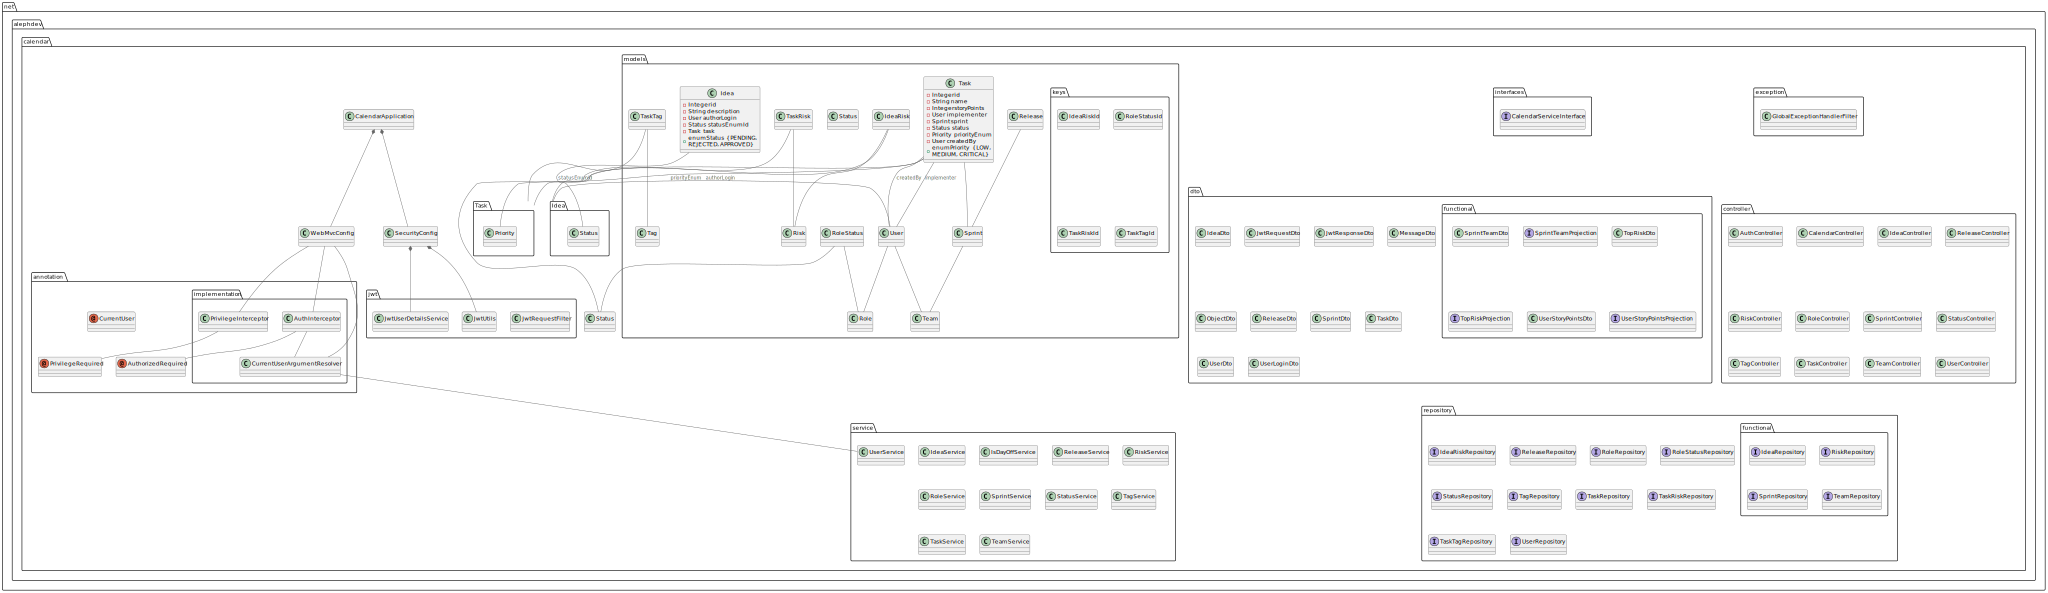
\includegraphics[width=.9\textwidth]{dia1}
\end{center}

\begin{center}
  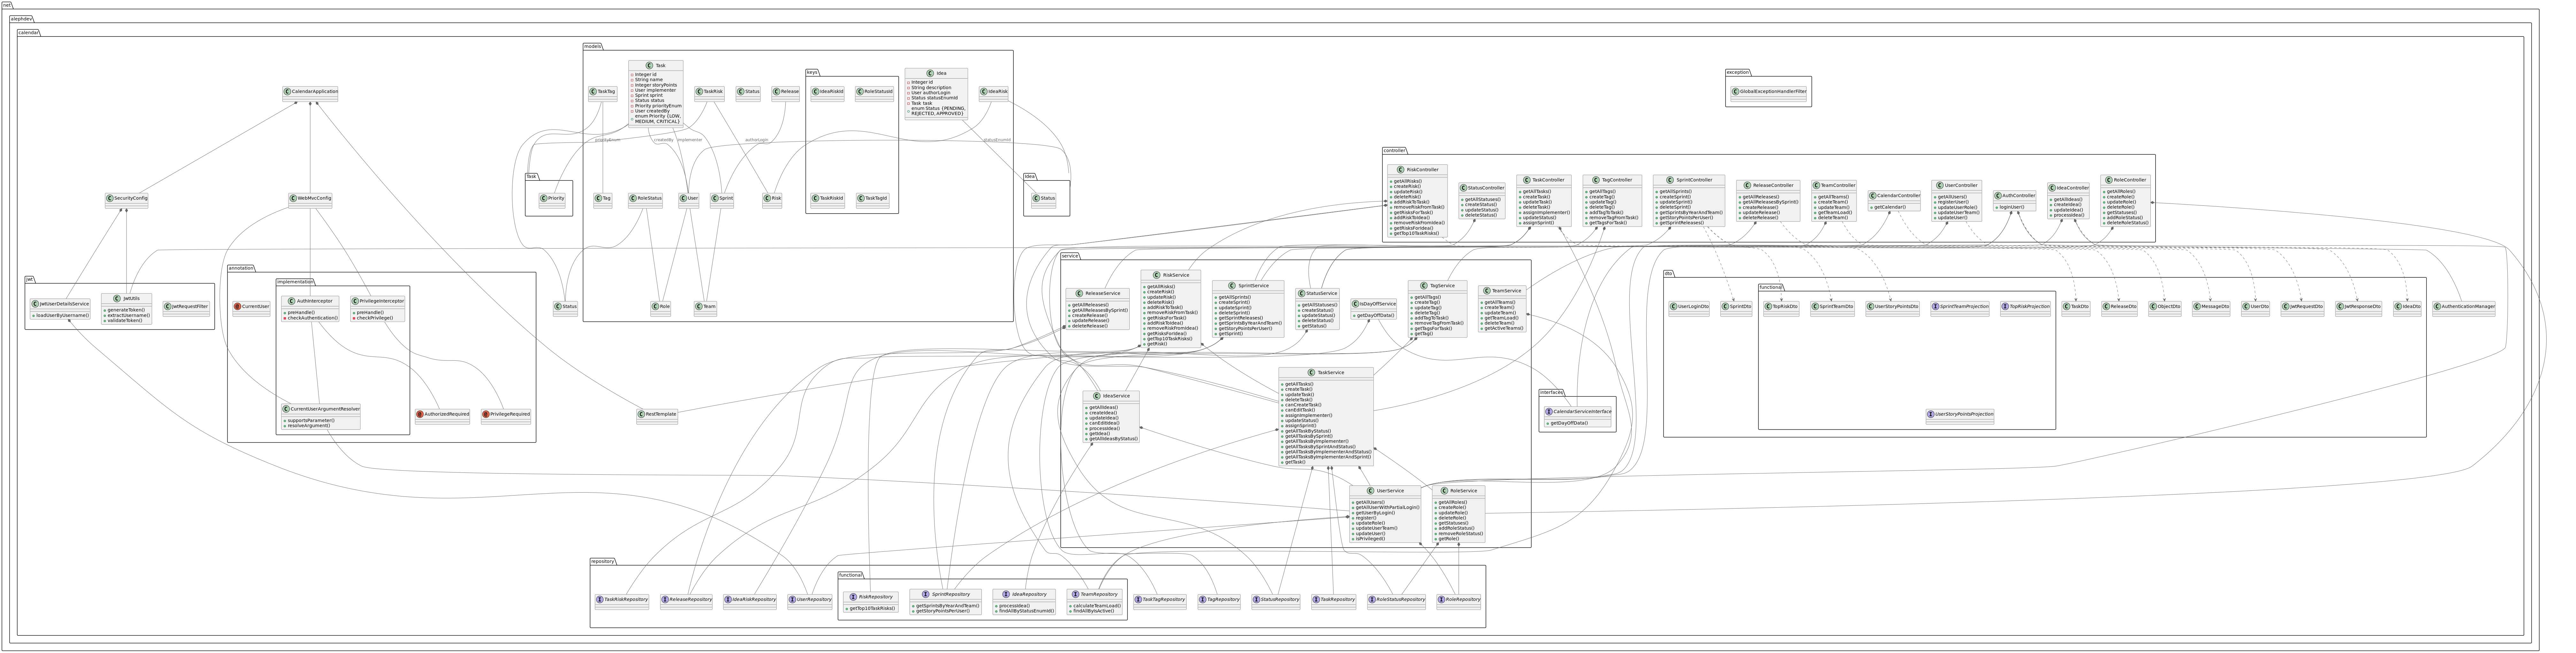
\includegraphics[width=.9\textwidth]{dia2}
\end{center}

\section{Рефакторинг инфраструктуры и развертывания}

Коммит: \texttt{d3a49cf} --- <<рефакторинг автоматического разворота>>

\subsubsection{Описание практики}
Выполнен рефакторинг процесса контейнеризации и автоматического развертывания приложения с использованием Docker и Docker Compose.
\subsubsection{Выполненные изменения}
\begin{itemize}
\item Добавлен файл \texttt{.dockerignore} для исключения ненужных файлов из Docker-образа
\item Улучшен \texttt{Dockerfile} --- оптимизирована многоэтапная сборка
\item Переработан \texttt{docker-compose.yml} --- улучшена конфигурация сервисов
\end{itemize}

\subsubsection{Применённые практики}
\begin{itemize}
\item \textbf{Multi-stage builds} --- использование многоэтапной сборки Docker для уменьшения размера образа
\item Последовательность команд для эффективного кеширования
\item Параметризация настроек приложения
\end{itemize}

\subsubsection{Важность для проекта}
\begin{enumerate}
\item Автоматизированный процесс сборки и запуска сокращает время развертывания
\item Гарантируется идентичность окружений разработки, тестирования и продакшена
\item Оптимизация Docker-образов снижает нагрузку на инфраструктуру и ускоряет доставку
\item Новые разработчики могут поднять проект одной командой
\end{enumerate}


\section{Рефакторинг структуры базы данных}

Коммит: \texttt{613271a} --- <<Отделение sql для инита>>

\subsubsection{Описание практики}
Проведена модульная реорганизация SQL-скриптов инициализации базы данных с разделением на логические компоненты.

\subsubsection{Выполненные изменения}
\begin{itemize}
\item Создана отдельная директория \texttt{postgres/} для всех SQL-скриптов
\item Монолитный файл разделён на модульные компоненты:
\begin{itemize}
\item \texttt{init-tables.sql}  --- создание таблиц
\item \texttt{init-constraints.sql} --- определение ограничений
\item \texttt{init-index.sql} --- создание индексов
\item \texttt{init-func.sql} --- функции базы данных
\item \texttt{init-procedure.sql} --- хранимые процедуры
\item \texttt{init-triggers.sql} --- триггеры
\item \texttt{init-inserts.sql} --- начальные данные
\item \texttt{init-pass.sql} --- инициализация паролей
\end{itemize}
\item Реорганизована структура проекта (перемещены диаграммы классов в отдельную папку)
\item Обновлён \texttt{application.yaml} для работы с новой структурой
\end{itemize}

\subsubsection{Применённые практики}
    \begin{itemize}
    \item \textbf{Separation of Concerns (SoC)} --- разделение ответственности на уровне SQL-скриптов
    \item \textbf{Single Responsibility Principle (SRP)} --- каждый файл отвечает за одну область БД
    \end{itemize}

\subsubsection{Важность для проекта}
    \begin{enumerate}
    \item Легко найти и модифицировать конкретный аспект схемы
    \item Точечные изменения в git-истории, простота code review
    \item Изменения в одном компоненте не влияют на другие
    \item Разные разработчики могут работать с разными файлами без конфликтов
    \end{enumerate}


\section{Внедрение стандартов качества кода}

Коммит: \texttt{e7c6774} --- <<Добавлена проверка при сборке проекта на соответствие стилю кода>>

\subsubsection{Описание практики}
Интегрирована автоматическая проверка соответствия кода стандартам Google Java Style Guide на этапе сборки проекта.

\subsubsection{Выполненные изменения}
    \begin{itemize}
    \item Добавлена зависимость \texttt{maven-checkstyle-plugin}
    \item Интегрированы конфигурационные файлы:
        \begin{itemize}
        \item \texttt{tools/checkstyle/google\_checks.xml} --- правила проверки кода
        \item \texttt{tools/checkstyle/eclipse-java-google-style.xml} --- конфигурация для IDE
        \end{itemize}
    \item Настроена автоматическая проверка при выполнении сборки
    \end{itemize}

\subsubsection{Применённые практики}
    \begin{itemize}
    \item \textbf{Static Code Analysis} --- статический анализ кода без его выполнения
    \item \textbf{Coding Standards} --- следование индустриальным стандартам (Google Style Guide)
    \item \textbf{Shift Left Testing} --- раннее обнаружение проблем на этапе сборки
    \item \textbf{Continuous Integration} --- автоматизация проверок качества кода
    \end{itemize}

\subsubsection{Важность для проекта}
    \begin{enumerate}
    \item Весь код проекта следует единому стилю, независимо от автора
    \item Часть проверок выполняется автоматически, экономя время команды
    \item Многие потенциальные проблемы обнаруживаются до попадания в репозиторий
    \item Стандартизированный код легче читать и понимать
    \item Проблемы выявляются и устраняются сразу, не накапливаясь
    \end{enumerate}

\section{Рефакторинг кодовой базы}

\subsection{Коммиты}
    \begin{itemize}
        \item \texttt{8722ded} --- <<Рефакторинг кода на стиль>>
        \item \texttt{403fa28} --- <<устранение проблем в коде для соответствия google style>>
    \end{itemize}

\subsubsection{Описание практики}
Проведён масштабный рефакторинг всей кодовой базы для приведения к стандартам Google Java Style Guide и применения лучших практик ООП.

\subsubsection{Выполненные изменения}

\textbf{Первый этап (8722ded) --- Общий рефакторинг:}
\begin{itemize}
    \item Затронутые области:
    \begin{itemize}
        \item \textbf{Конфигурация безопасности} (\texttt{SecurityConfig.java}, \texttt{WebMvcConfig.java}, \texttt{WebSocketConfig.java})
        \item \textbf{Контроллеры} --- все 13 контроллеров (Auth, Calendar, Idea, Release, Risk, Role, Sprint, Status, Tag, Task, Team, User)
        \item \textbf{Модели данных} --- все 15 entity-классов
        \item \textbf{DTO} --- 12 классов передачи данных
        \item \textbf{Сервисы} --- все 10 сервисных классов
        \item \textbf{Репозитории} --- функциональные репозитории и спецификации
        \item \textbf{Обработка исключений} (\texttt{GlobalExceptionHandlerFilter})
        \item \textbf{JWT-аутентификация} (\texttt{JwtRequestFilter}, \texttt{JwtUtils}, \texttt{JwtUserDetailsService})
    \end{itemize}
\end{itemize}

\textbf{Второй этап (403fa28) --- Устранение проблем:}
\begin{itemize}
    \item Устранение оставшихся нарушений стиля в 30 файлах
    \item Исправление предупреждений Checkstyle, которые не правятся автоматически
\end{itemize}

\subsubsection{Применённые практики}
\begin{itemize}
    \item \textbf{Consistent Indentation} --- единообразные отступы (2 пробела)
    \item \textbf{Line Length Limit} --- ограничение длины строки (100 символов)
    \item \textbf{Import Organization} --- правильная организация импортов
    \item \textbf{Naming Conventions} --- соблюдение конвенций именования (camelCase, PascalCase)
\end{itemize}
\begin{itemize}
    \item \textbf{DRY (Don't Repeat Yourself)} --- устранение дублирования кода
    \item \textbf{Clean Code} --- применение принципов чистого кода
\end{itemize}

\section{Документирование API через OpenAPI}

\subsection{Коммиты}
    \begin{itemize}
        \item \texttt{0935443} --- <<openapi config>>
        \item \texttt{9134f3a} --- <<functional dtos schemas>>
        \item \texttt{6887adf} --- <<general dtos schemas>>
        \item \texttt{f703de0} --- <<all controllers schemas>>
    \end{itemize}

\subsubsection{Описание практики}
Внедрена полная документация REST API с использованием спецификации OpenAPI 3.0 (Swagger), включающая аннотирование всех контроллеров, методов и моделей данных.

\subsubsection{Выполненные изменения}
\textbf{Этап 1 --- Конфигурация OpenAPI (0935443)}\\
\textbf{Этап 2 --- Документирование Functional DTOs (9134f3a):}

Добавлены аннотации \texttt{@Schema} для специализированных DTO:
\begin{itemize}
\item \texttt{SprintTeamDto} --- данные о команде спринта
\item \texttt{TopRiskDto} --- информация о главных рисках
\item \texttt{UserStoryPointsDto} --- статистика story points пользователей
\end{itemize}
\textbf{Этап 3 --- Документирование General DTOs (6887adf):}
\begin{itemize}
\item \texttt{IdeaDto}, \texttt{ReleaseDto}, \texttt{SprintDto}, \texttt{TaskDto}, \texttt{UserDto} --- основные сущности
\item \texttt{JwtRequestDto}, \texttt{JwtResponseDto} --- аутентификация
\item \texttt{MessageDto} --- системные сообщения
\end{itemize}
\textbf{Этап 4 --- Документирование контроллеров (f703de0):}
\begin{itemize}
\item \textbf{Аннотации контроллеров:} \texttt{@Tag} для группировки endpoints
\item \textbf{Аннотации методов:} \texttt{@Operation} с описанием каждой операции
\item \textbf{Аннотации параметров:} \texttt{@Parameter} для query, path и body параметров
\item \textbf{Аннотации ответов:} \texttt{@ApiResponse} для всех возможных HTTP-статусов
\item \textbf{Схемы безопасности:} \texttt{@SecurityRequirement} для защищённых endpoints
\end{itemize}

\subsubsection{Применённые практики}
\begin{itemize}
\item \textbf{OpenAPI Specification} --- использование индустриального стандарта документирования API
\item \textbf{Self-Documenting Code} --- код документирует сам себя через аннотации
\item \textbf{API-First Design} --- явное описание контракта API
\end{itemize}

\subsubsection{Важность для проекта}

\textbf{Для разработки:}
\begin{enumerate}
\item \textbf{Contract-First Development} --- чёткий контракт между frontend и backend
\item \textbf{Reduced Communication Overhead} --- меньше вопросов между командами
\item \textbf{API Testing} --- возможность тестирования API прямо из браузера
\item \textbf{Mock Generation} --- автоматическая генерация моков для тестирования
\end{enumerate}
\textbf{Для команды:}
\begin{enumerate}[resume]
\item \textbf{Onboarding} --- новые разработчики быстро понимают структуру API
\item \textbf{Knowledge Sharing} --- документация доступна всем участникам команды
\item \textbf{Consistency} --- единообразное понимание API всеми разработчиками
\end{enumerate}
\textbf{Для проекта:}
\begin{enumerate}[resume]
\item \textbf{Professional Standard} --- использование индустриальных стандартов
\item \textbf{Integration Ready} --- легкая интеграция с внешними системами
\item \textbf{API Discovery} --- возможность исследования API через Swagger UI
\item \textbf{Reduced Documentation Debt} --- документация поддерживается автоматически вместе с кодом
\item \textbf{Quality Assurance} --- явное описание ожидаемого поведения упрощает тестирование
\end{enumerate}

\section{Итоги и результаты}

При каждой фазе рефакторинга проект стновилось легче и легче просматривать, развивать. Данная работа помогла структурировать практически мертвый для разворота и разработки проект. 

\end{document}

\begin{center}
  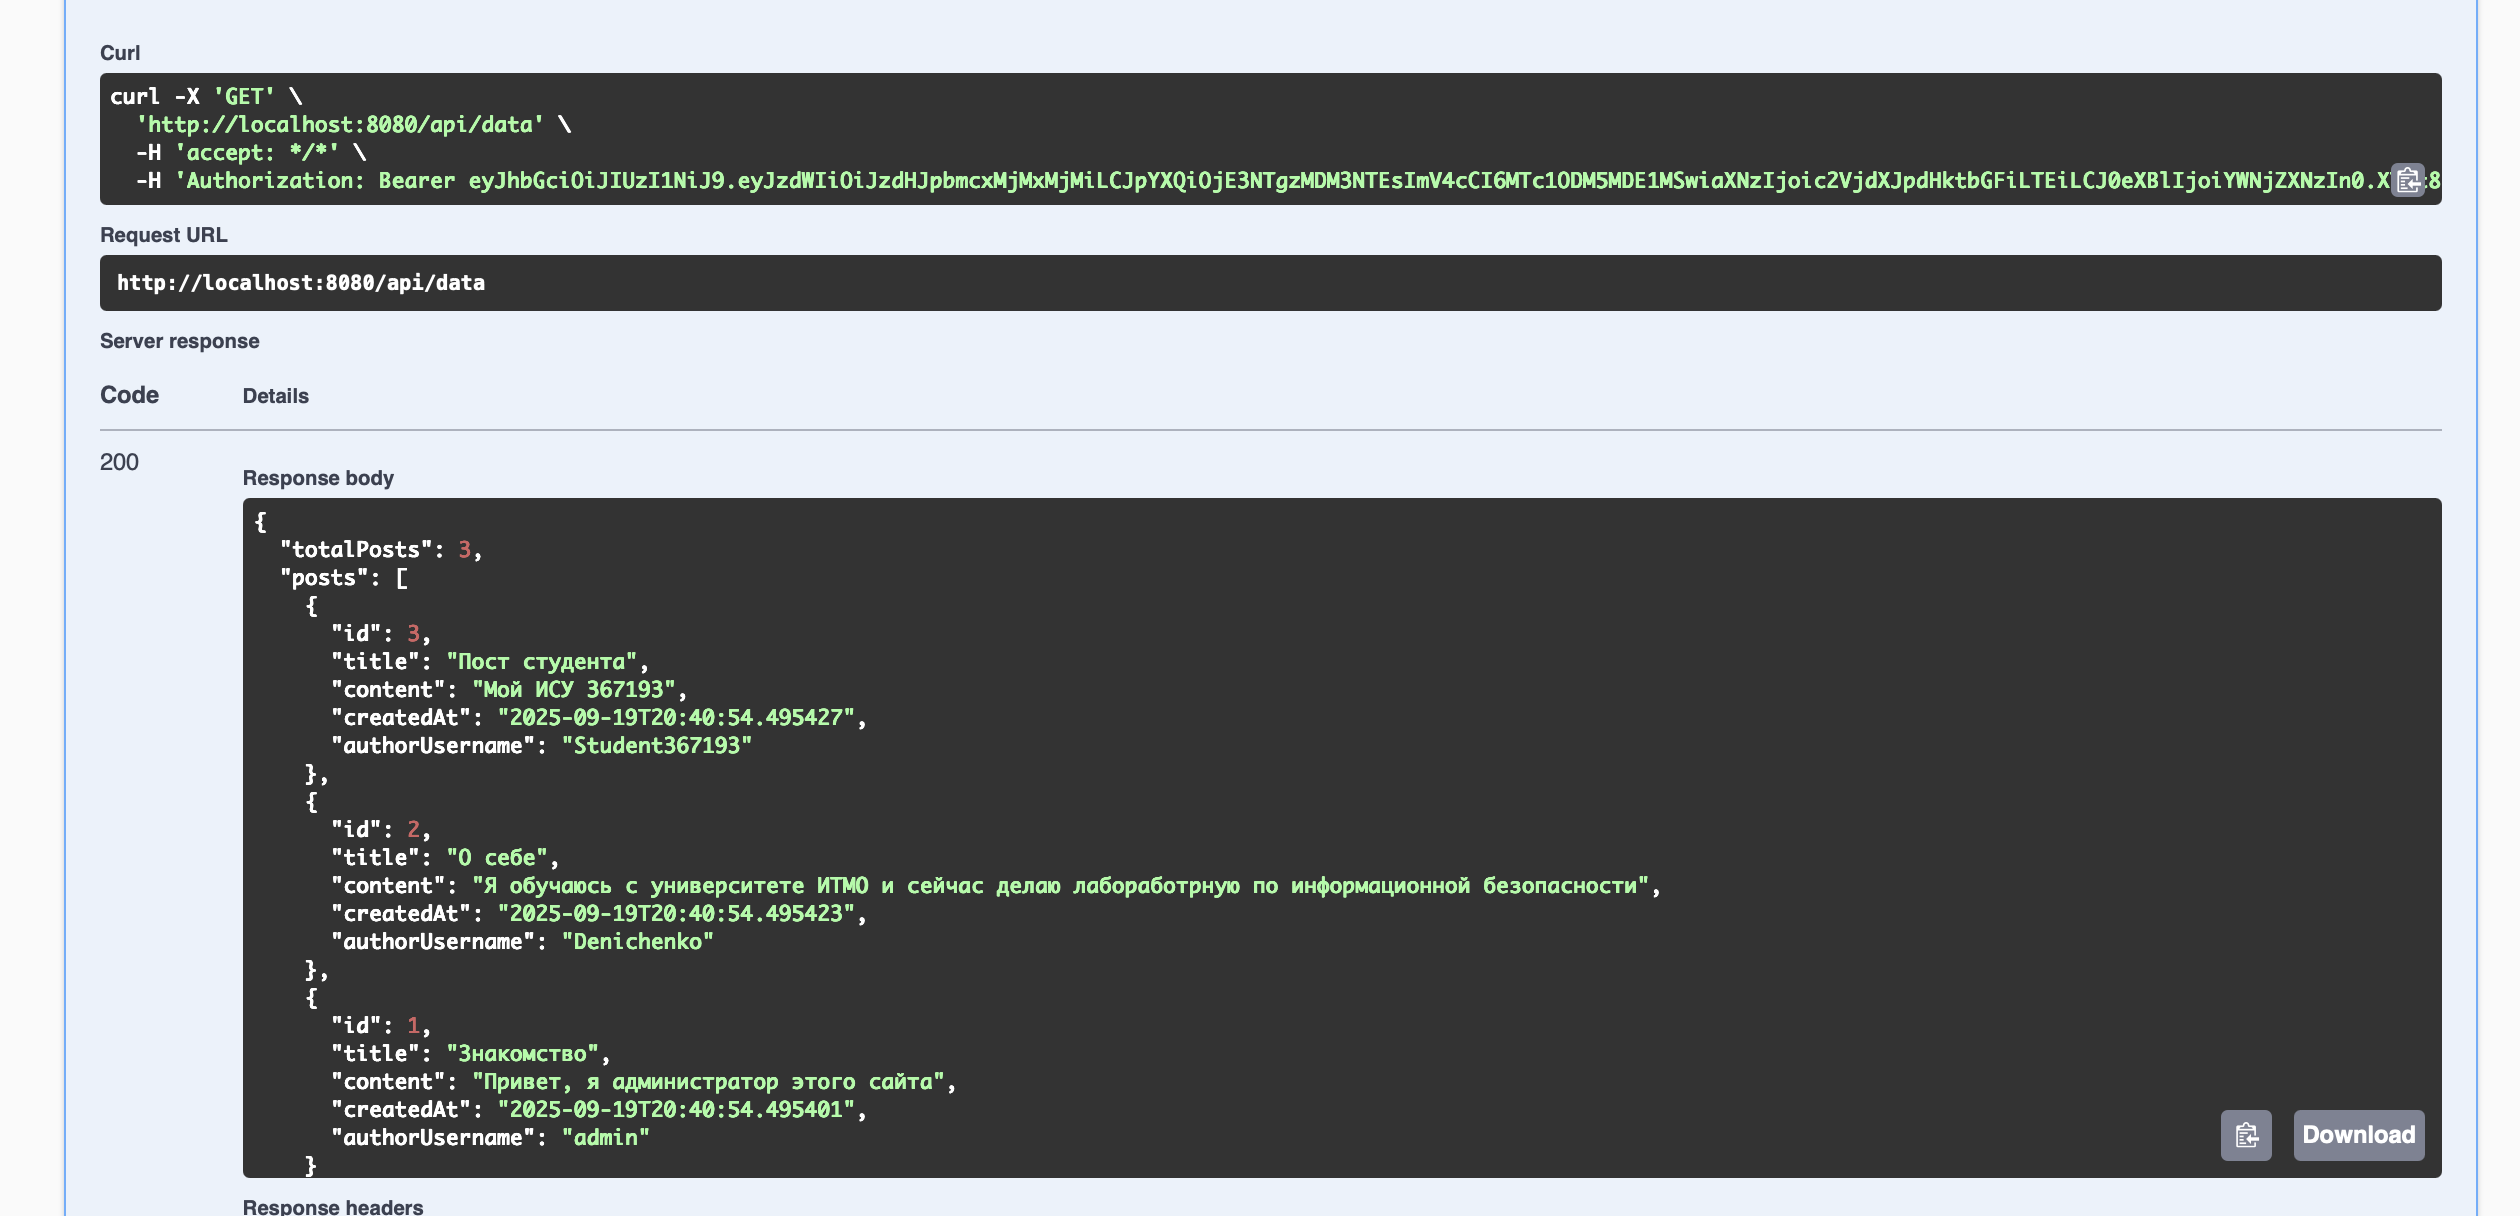
\includegraphics[width=.9\textwidth]{posts}
\end{center}

\href{https://github.com/Alex-de-bug/security-lab-1/actions/runs/17864752066}{Последний верный CI} (https://github.com/Alex-de-bug/security-lab-1/actions/runs/17864752066)
http://testaspnet.vulnweb.com